\begin{figure*}
    \centering
    \begin{subfigure}[t]{0.035\textwidth}
        \vspace{0px}
        \centering
        \rotatebox{90}{\small\clean\hspace*{0.5cm}}
    \end{subfigure}
    \begin{subfigure}[t]{0.115\textwidth}
        \vspace{0px}
        \centering
        \small Mesh/SDF\\
        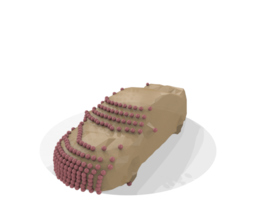
\includegraphics[width=1.75cm,trim={0.5cm 0.75cm 1.5cm 1.5cm},clip]{gfx/experiments_data/clean*/simplified/00003}
    \end{subfigure}
    \begin{subfigure}[t]{0.115\textwidth}
        \vspace{0px}
        \centering
        \small Occupancy\\
        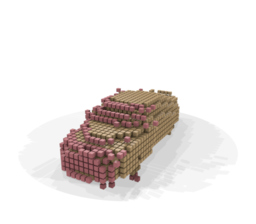
\includegraphics[width=1.75cm,trim={0.5cm 0.75cm 1.5cm 1.5cm},clip]{gfx/experiments_data/clean/voxelized/00003}
    \end{subfigure}
    \begin{subfigure}[t]{0.115\textwidth}
        \vspace{0px}
        \centering
        \small Mesh/SDF\\
        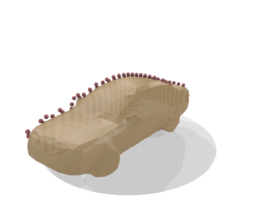
\includegraphics[width=1.75cm,trim={0.5cm 0.75cm 1.5cm 1.5cm},clip]{gfx/experiments_data/clean*/simplified/00009}
    \end{subfigure}
    \begin{subfigure}[t]{0.115\textwidth}
        \vspace{0px}
        \centering
        \small Occupancy\\
        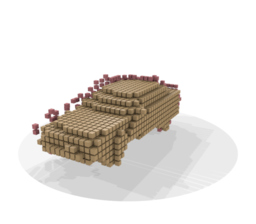
\includegraphics[width=1.75cm,trim={0.5cm 0.75cm 1.5cm 1.5cm},clip]{gfx/experiments_data/clean/voxelized/00009}
    \end{subfigure}
    \begin{subfigure}[t]{0.115\textwidth}
        \vspace{0px}
        \centering
        \small Mesh/SDF\\
        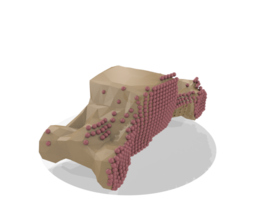
\includegraphics[width=1.75cm,trim={0.5cm 0.75cm 1.5cm 1.5cm},clip]{gfx/experiments_data/clean*/simplified/00023}
    \end{subfigure}
    \begin{subfigure}[t]{0.115\textwidth}
        \vspace{0px}
        \centering
        \small Occupancy\\
        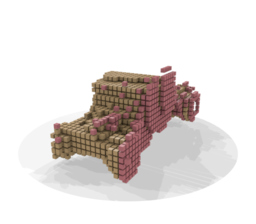
\includegraphics[width=1.75cm,trim={0.5cm 0.75cm 1.5cm 1.5cm},clip]{gfx/experiments_data/clean/voxelized/00023}
    \end{subfigure}
    \begin{subfigure}[t]{0.115\textwidth}
        \vspace{0px}
        \centering
        \small Mesh/SDF\\
        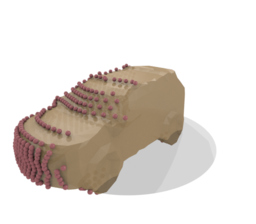
\includegraphics[width=1.75cm,trim={0.5cm 0.75cm 1.5cm 1.5cm},clip]{gfx/experiments_data/clean*/simplified/00010}
    \end{subfigure}
    \begin{subfigure}[t]{0.115\textwidth}
        \vspace{0px}
        \centering
        \small Occupancy\\
        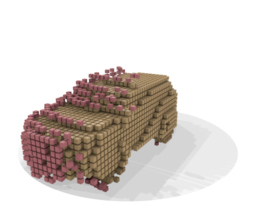
\includegraphics[width=1.75cm,trim={0.5cm 0.75cm 1.5cm 1.5cm},clip]{gfx/experiments_data/clean/voxelized/00010}
    \end{subfigure}\\
    \begin{subfigure}[t]{0.035\textwidth}
        \vspace{0px}
        \centering
        \rotatebox{90}{\small\clean\hspace*{0.3cm}}
    \end{subfigure}
    \begin{subfigure}[t]{0.115\textwidth}
        \vspace{0px}
        \centering
        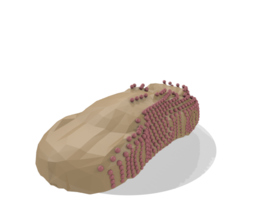
\includegraphics[width=1.75cm,trim={0.5cm 0.75cm 1.5cm 1.5cm},clip]{gfx/experiments_data/clean*/simplified/00002}
    \end{subfigure}
    \begin{subfigure}[t]{0.115\textwidth}
        \vspace{0px}
        \centering
        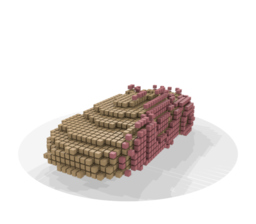
\includegraphics[width=1.75cm,trim={0.5cm 0.75cm 1.5cm 1.5cm},clip]{gfx/experiments_data/clean/voxelized/00002}
    \end{subfigure}
    \begin{subfigure}[t]{0.115\textwidth}
        \vspace{0px}
        \centering
        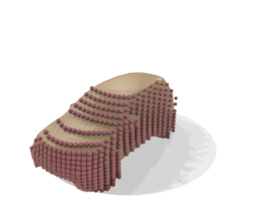
\includegraphics[width=1.75cm,trim={0.5cm 0.75cm 1.5cm 1.5cm},clip]{gfx/experiments_data/clean*/simplified/00007}
    \end{subfigure}
    \begin{subfigure}[t]{0.115\textwidth}
        \vspace{0px}
        \centering
        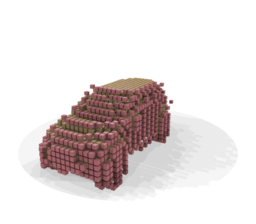
\includegraphics[width=1.75cm,trim={0.5cm 0.75cm 1.5cm 1.5cm},clip]{gfx/experiments_data/clean/voxelized/00007}
    \end{subfigure}
    \begin{subfigure}[t]{0.115\textwidth}
        \vspace{0px}
        \centering
        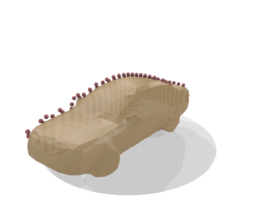
\includegraphics[width=1.75cm,trim={0.5cm 0.75cm 1.5cm 1.5cm},clip]{gfx/experiments_data/clean*/simplified/00009}
    \end{subfigure}
    \begin{subfigure}[t]{0.115\textwidth}
        \vspace{0px}
        \centering
        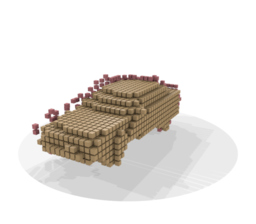
\includegraphics[width=1.75cm,trim={0.5cm 0.75cm 1.5cm 1.5cm},clip]{gfx/experiments_data/clean/voxelized/00009}
    \end{subfigure}
    \begin{subfigure}[t]{0.115\textwidth}
        \vspace{0px}
        \centering
        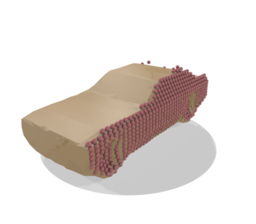
\includegraphics[width=1.75cm,trim={0.5cm 0.75cm 1.5cm 1.5cm},clip]{gfx/experiments_data/clean*/simplified/00013}
    \end{subfigure}
    \begin{subfigure}[t]{0.115\textwidth}
        \vspace{0px}
        \centering
        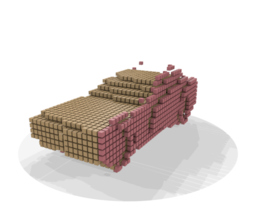
\includegraphics[width=1.75cm,trim={0.5cm 0.75cm 1.5cm 1.5cm},clip]{gfx/experiments_data/clean/voxelized/00013}
    \end{subfigure}\\
    
    \begin{subfigure}[t]{0.035\textwidth}
        \vspace{0px}
        \centering
        \rotatebox{90}{\small\noisy\hspace*{0.3cm}}
    \end{subfigure}
    \begin{subfigure}[t]{0.115\textwidth}
        \vspace{0px}
        \centering
        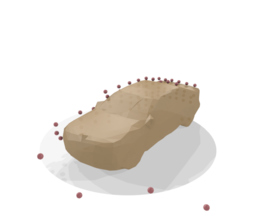
\includegraphics[width=1.75cm,trim={0.5cm 0.75cm 1.5cm 1.5cm},clip]{gfx/experiments_data/noisy*/simplified/00021}
    \end{subfigure}
    \begin{subfigure}[t]{0.115\textwidth}
        \vspace{0px}
        \centering
        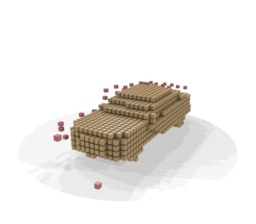
\includegraphics[width=1.75cm,trim={0.5cm 0.75cm 1.5cm 1.5cm},clip]{gfx/experiments_data/noisy/voxelized/00021}
    \end{subfigure}
    \begin{subfigure}[t]{0.115\textwidth}
        \vspace{0px}
        \centering
        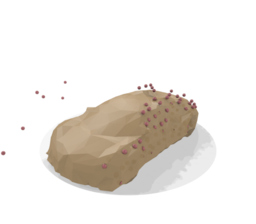
\includegraphics[width=1.75cm,trim={0.5cm 0.75cm 1.5cm 1.5cm},clip]{gfx/experiments_data/noisy*/simplified/00008}
    \end{subfigure}
    \begin{subfigure}[t]{0.115\textwidth}
        \vspace{0px}
        \centering
        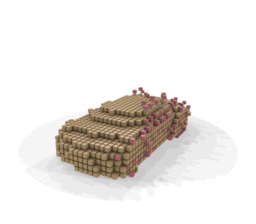
\includegraphics[width=1.75cm,trim={0.5cm 0.75cm 1.5cm 1.5cm},clip]{gfx/experiments_data/noisy/voxelized/00008}
    \end{subfigure}
    \begin{subfigure}[t]{0.115\textwidth}
        \vspace{0px}
        \centering
        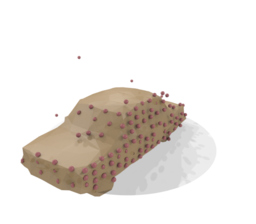
\includegraphics[width=1.75cm,trim={0.5cm 0.75cm 1.5cm 1.5cm},clip]{gfx/experiments_data/noisy*/simplified/00004}
    \end{subfigure}
    \begin{subfigure}[t]{0.115\textwidth}
        \vspace{0px}
        \centering
        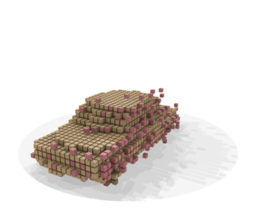
\includegraphics[width=1.75cm,trim={0.5cm 0.75cm 1.5cm 1.5cm},clip]{gfx/experiments_data/noisy/voxelized/00004}
    \end{subfigure}
    \begin{subfigure}[t]{0.115\textwidth}
        \vspace{0px}
        \centering
        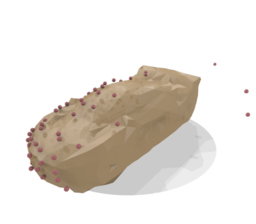
\includegraphics[width=1.75cm,trim={0.5cm 0.75cm 1.5cm 1.5cm},clip]{gfx/experiments_data/noisy*/simplified/00012}
    \end{subfigure}
    \begin{subfigure}[t]{0.115\textwidth}
        \vspace{0px}
        \centering
        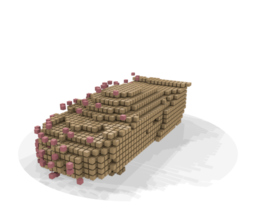
\includegraphics[width=1.75cm,trim={0.5cm 0.75cm 1.5cm 1.5cm},clip]{gfx/experiments_data/noisy/voxelized/00012}
    \end{subfigure}\\
    \begin{subfigure}[t]{0.035\textwidth}
        \vspace{0px}
        \centering
        \rotatebox{90}{\small\noisy\hspace*{0.3cm}}
    \end{subfigure}
    \begin{subfigure}[t]{0.115\textwidth}
        \vspace{0px}
        \centering
        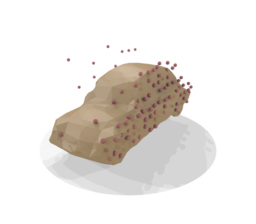
\includegraphics[width=1.75cm,trim={0.5cm 0.75cm 1.5cm 1.5cm},clip]{gfx/experiments_data/noisy*/simplified/00015}
    \end{subfigure}
    \begin{subfigure}[t]{0.115\textwidth}
        \vspace{0px}
        \centering
        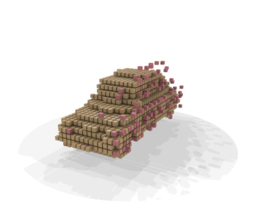
\includegraphics[width=1.75cm,trim={0.5cm 0.75cm 1.5cm 1.5cm},clip]{gfx/experiments_data/noisy/voxelized/00015}
    \end{subfigure}
    \begin{subfigure}[t]{0.115\textwidth}
        \vspace{0px}
        \centering
        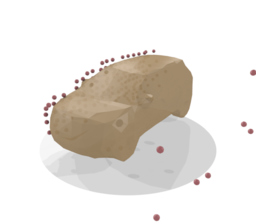
\includegraphics[width=1.75cm,trim={0.5cm 0.75cm 1.5cm 1.5cm},clip]{gfx/experiments_data/noisy*/simplified/00019}
    \end{subfigure}
    \begin{subfigure}[t]{0.115\textwidth}
        \vspace{0px}
        \centering
        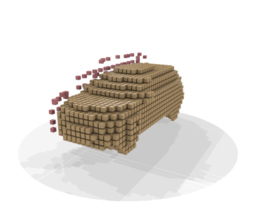
\includegraphics[width=1.75cm,trim={0.5cm 0.75cm 1.5cm 1.5cm},clip]{gfx/experiments_data/noisy/voxelized/00019}
    \end{subfigure}
    \begin{subfigure}[t]{0.115\textwidth}
        \vspace{0px}
        \centering
        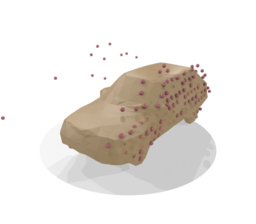
\includegraphics[width=1.75cm,trim={0.5cm 0.75cm 1.5cm 1.5cm},clip]{gfx/experiments_data/noisy*/simplified/00017}
    \end{subfigure}
    \begin{subfigure}[t]{0.115\textwidth}
        \vspace{0px}
        \centering
        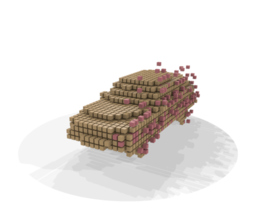
\includegraphics[width=1.75cm,trim={0.5cm 0.75cm 1.5cm 1.5cm},clip]{gfx/experiments_data/noisy/voxelized/00017}
    \end{subfigure}
    \begin{subfigure}[t]{0.115\textwidth}
        \vspace{0px}
        \centering
        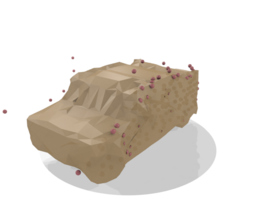
\includegraphics[width=1.75cm,trim={0.5cm 0.75cm 1.5cm 1.5cm},clip]{gfx/experiments_data/noisy*/simplified/00016}
    \end{subfigure}
    \begin{subfigure}[t]{0.115\textwidth}
        \vspace{0px}
        \centering
        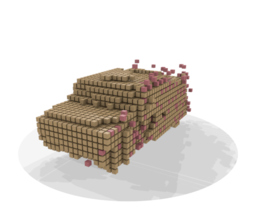
\includegraphics[width=1.75cm,trim={0.5cm 0.75cm 1.5cm 1.5cm},clip]{gfx/experiments_data/noisy/voxelized/00016}
    \end{subfigure}\\
    \vspace{0.5cm}
    \begin{subfigure}[t]{0.035\textwidth}
        \vspace{0px}
        \centering
        \rotatebox{90}{\small KITTI\hspace*{0.5cm}}
    \end{subfigure}
    \begin{subfigure}[t]{0.115\textwidth}
        \vspace{0px}
        \centering
        \small Observation\\
        
\includegraphics[width=1.75cm,trim={0.5cm 0.75cm 1.5cm 1.5cm},clip]{gfx/experiments_data/kitti*/points/00012}
    \end{subfigure}
    \begin{subfigure}[t]{0.115\textwidth}
        \vspace{0px}
        \centering
        \small GT\\
        
\includegraphics[width=1.75cm,trim={0.5cm 0.75cm 1.5cm 1.5cm},clip]{gfx/experiments_data/kitti*/gt/00012}
    \end{subfigure}
    \begin{subfigure}[t]{0.115\textwidth}
        \vspace{0px}
        \centering
        \small Observation\\
        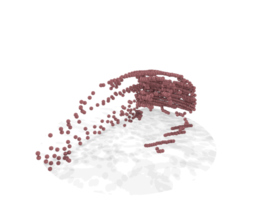
\includegraphics[width=1.75cm,trim={0.5cm 0.75cm 1.5cm 1.5cm},clip]{gfx/experiments_data/kitti*/points/00045}
    \end{subfigure}
    \begin{subfigure}[t]{0.115\textwidth}
        \vspace{0px}
        \centering
        \small GT\\
        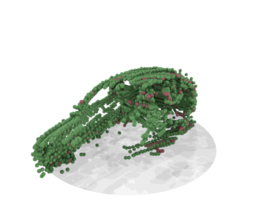
\includegraphics[width=1.75cm,trim={0.5cm 0.75cm 1.5cm 1.5cm},clip]{gfx/experiments_data/kitti*/gt/00045}
    \end{subfigure}
    \begin{subfigure}[t]{0.115\textwidth}
        \vspace{0px}
        \centering
        \small Observation\\
        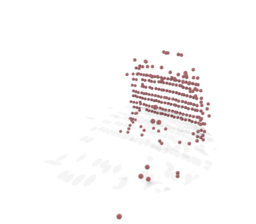
\includegraphics[width=1.75cm,trim={0.5cm 0.75cm 1.5cm 1.5cm},clip]{gfx/experiments_data/kitti*/points/00047}
    \end{subfigure}
    \begin{subfigure}[t]{0.115\textwidth}
        \vspace{0px}
        \centering
        \small GT\\
        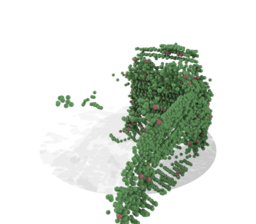
\includegraphics[width=1.75cm,trim={0.5cm 0.75cm 1.5cm 1.5cm},clip]{gfx/experiments_data/kitti*/gt/00047}
    \end{subfigure}
    \begin{subfigure}[t]{0.115\textwidth}
        \vspace{0px}
        \centering
        Observation\\
        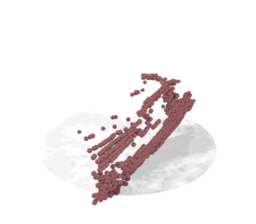
\includegraphics[width=1.75cm,trim={0.5cm 0.75cm 1.5cm 1.5cm},clip]{gfx/experiments_data/kitti*/points/00010}
    \end{subfigure}
    \begin{subfigure}[t]{0.115\textwidth}
        \vspace{0px}
        \centering
        \small GT\\
        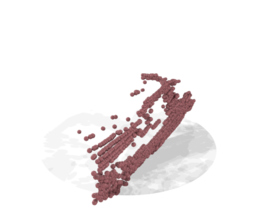
\includegraphics[width=1.75cm,trim={0.5cm 0.75cm 1.5cm 1.5cm},clip]{gfx/experiments_data/kitti*/gt/00010}
    \end{subfigure}
    \begin{subfigure}[t]{0.035\textwidth}
        \vspace{0px}
        \centering
        \rotatebox{90}{\small KITTI\hspace*{0.5cm}}
    \end{subfigure}
    \begin{subfigure}[t]{0.115\textwidth}
        \vspace{0px}
        \centering
        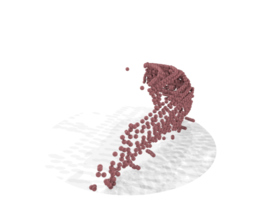
\includegraphics[width=1.75cm,trim={0.5cm 0.75cm 1.5cm 1.5cm},clip]{gfx/experiments_data/kitti*/points/00020}
    \end{subfigure}
    \begin{subfigure}[t]{0.115\textwidth}
        \vspace{0px}
        \centering
        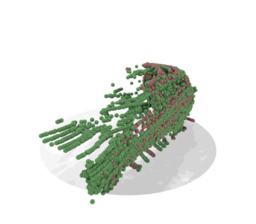
\includegraphics[width=1.75cm,trim={0.5cm 0.75cm 1.5cm 1.5cm},clip]{gfx/experiments_data/kitti*/gt/00020}
    \end{subfigure}
    \begin{subfigure}[t]{0.115\textwidth}
        \vspace{0px}
        \centering
        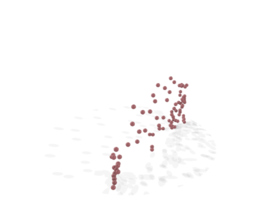
\includegraphics[width=1.75cm,trim={0.5cm 0.75cm 1.5cm 1.5cm},clip]{gfx/experiments_data/kitti*/points/00024}
    \end{subfigure}
    \begin{subfigure}[t]{0.115\textwidth}
        \vspace{0px}
        \centering
        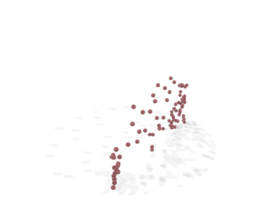
\includegraphics[width=1.75cm,trim={0.5cm 0.75cm 1.5cm 1.5cm},clip]{gfx/experiments_data/kitti*/gt/00024}
    \end{subfigure}
    \begin{subfigure}[t]{0.115\textwidth}
        \vspace{0px}
        \centering
        
\includegraphics[width=1.75cm,trim={0.5cm 0.75cm 1.5cm 1.5cm},clip]{gfx/experiments_data/kitti*/points/00028}
    \end{subfigure}
    \begin{subfigure}[t]{0.115\textwidth}
        \vspace{0px}
        \centering
        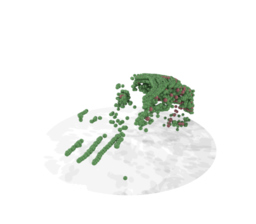
\includegraphics[width=1.75cm,trim={0.5cm 0.75cm 1.5cm 1.5cm},clip]{gfx/experiments_data/kitti*/gt/00028}
    \end{subfigure}
    \begin{subfigure}[t]{0.115\textwidth}
        \vspace{0px}
        \centering
        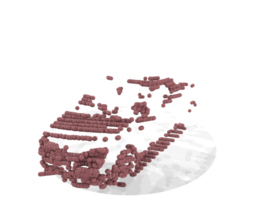
\includegraphics[width=1.75cm,trim={0.5cm 0.75cm 1.5cm 1.5cm},clip]{gfx/experiments_data/kitti*/points/00038}
    \end{subfigure}
    \begin{subfigure}[t]{0.115\textwidth}
        \vspace{0px}
        \centering
        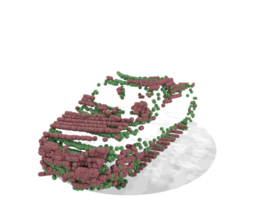
\includegraphics[width=1.75cm,trim={0.5cm 0.75cm 1.5cm 1.5cm},clip]{gfx/experiments_data/kitti*/gt/00038}
    \end{subfigure}\\
    \vspace{0.5cm}
    \begin{subfigure}[t]{0.035\textwidth}
    	\vspace{0px}
    	\centering
    	\rotatebox{90}{\small ModelNet\hspace*{0.25cm}}
    \end{subfigure}
    \begin{subfigure}[t]{0.115\textwidth}
    	\vspace{0px}
    	\centering
    	\small Observation\\
    	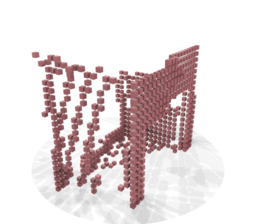
\includegraphics[width=1.75cm,trim={1cm 0cm 0.75cm 1cm},clip]{gfx/experiments_modelnet/vae_occ_aml/bdmnsf.clean.25.small.weighted/points/00023}
    \end{subfigure}
    \begin{subfigure}[t]{0.115\textwidth}
    	\vspace{0px}
    	\centering
    	\small Occupancy\\
    	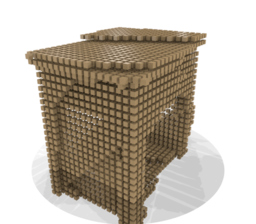
\includegraphics[width=1.75cm,trim={1cm 0cm 0.75cm 1cm},clip]{gfx/experiments_modelnet/vae_occ_aml/bdmnsf.clean.25.small.weighted/target/00023}
    \end{subfigure}
    \begin{subfigure}[t]{0.115\textwidth}
        \vspace{0px}
        \centering
        \small Observation\\
        \includegraphics[width=1.75cm,trim={1cm 0cm 0.75cm 1cm},clip]{gfx/experiments_modelnet/vae_occ_aml/bdmnsf.clean.25.small.weighted/points/00014}
    \end{subfigure}
    \begin{subfigure}[t]{0.115\textwidth}
        \vspace{0px}
        \centering
        \small Occupancy\\
        \includegraphics[width=1.75cm,trim={1cm 0cm 0.75cm 1cm},clip]{gfx/experiments_modelnet/vae_occ_aml/bdmnsf.clean.25.small.weighted/target/00014}
    \end{subfigure}
    \begin{subfigure}[t]{0.115\textwidth}
        \vspace{0px}
        \centering
        \small Observation\\
        \includegraphics[width=1.75cm,trim={1cm 0cm 0.75cm 1cm},clip]{gfx/experiments_modelnet/vae_occ_aml/bdmnsf.clean.25.small.weighted/points/00002}
    \end{subfigure}
    \begin{subfigure}[t]{0.115\textwidth}
        \vspace{0px}
        \centering
        \small Occupancy\\
        \includegraphics[width=1.75cm,trim={1cm 0cm 0.75cm 1cm},clip]{gfx/experiments_modelnet/vae_occ_aml/bdmnsf.clean.25.small.weighted/target/00002}
    \end{subfigure}
    \begin{subfigure}[t]{0.115\textwidth}
        \vspace{0px}
        \centering
        \small Observation\\
        \includegraphics[width=1.75cm,trim={1cm 0cm 0.75cm 1cm},clip]{gfx/experiments_modelnet/vae_occ_aml/bdmnsf.clean.25.small.weighted/points/00006}
    \end{subfigure}
    \begin{subfigure}[t]{0.115\textwidth}
        \vspace{0px}
        \centering
        \small Occupancy\\
        \includegraphics[width=1.75cm,trim={1cm 0cm 0.75cm 1cm},clip]{gfx/experiments_modelnet/vae_occ_aml/bdmnsf.clean.25.small.weighted/target/00006}
    \end{subfigure}
    \begin{subfigure}[t]{0.035\textwidth}
        \vspace{0px}
        \centering
        \rotatebox{90}{\small ModelNet\hspace*{0.25cm}}
    \end{subfigure}
    \begin{subfigure}[t]{0.115\textwidth}
        \vspace{0px}
        \centering
        \includegraphics[width=1.75cm,trim={1cm 0cm 0.75cm 1cm},clip]{gfx/experiments_modelnet/vae_occ_aml/bdmnsf.clean.25.small.weighted/points/00008}
    \end{subfigure}
    \begin{subfigure}[t]{0.115\textwidth}
        \vspace{0px}
        \centering
        \includegraphics[width=1.75cm,trim={1cm 0cm 0.75cm 1cm},clip]{gfx/experiments_modelnet/vae_occ_aml/bdmnsf.clean.25.small.weighted/target/00008}
    \end{subfigure}
    \begin{subfigure}[t]{0.115\textwidth}
        \vspace{0px}
        \centering
        \includegraphics[width=1.75cm,trim={1cm 0cm 0.75cm 1cm},clip]{gfx/experiments_modelnet/vae_occ_aml/bdmnsf.clean.25.small.weighted/points/00022}
    \end{subfigure}
    \begin{subfigure}[t]{0.115\textwidth}
        \vspace{0px}
        \centering
        \includegraphics[width=1.75cm,trim={1cm 0cm 0.75cm 1cm},clip]{gfx/experiments_modelnet/vae_occ_aml/bdmnsf.clean.25.small.weighted/target/00022}
    \end{subfigure}
    \begin{subfigure}[t]{0.115\textwidth}
        \vspace{0px}
        \centering
        \includegraphics[width=1.75cm,trim={1cm 0cm 0.75cm 1cm},clip]{gfx/experiments_modelnet/vae_occ_aml/bdmnsf.clean.25.small.weighted/points/00007}
    \end{subfigure}
    \begin{subfigure}[t]{0.115\textwidth}
        \vspace{0px}
        \centering
        \includegraphics[width=1.75cm,trim={1cm 0cm 0.75cm 1cm},clip]{gfx/experiments_modelnet/vae_occ_aml/bdmnsf.clean.25.small.weighted/target/00007}
    \end{subfigure}
    \begin{subfigure}[t]{0.115\textwidth}
        \vspace{0px}
        \centering
        \includegraphics[width=1.75cm,trim={1cm 0cm 0.75cm 1cm},clip]{gfx/experiments_modelnet/vae_occ_aml/bdmnsf.clean.25.small.weighted/points/00019}
    \end{subfigure}
    \begin{subfigure}[t]{0.115\textwidth}
        \vspace{0px}
        \centering
        \includegraphics[width=1.75cm,trim={1cm 0cm 0.75cm 1cm},clip]{gfx/experiments_modelnet/vae_occ_aml/bdmnsf.clean.25.small.weighted/target/00019}
    \end{subfigure}
    \caption{{\bf Samples from our Datasets.} From top to bottom: \clean, \noisy, KITTI and ModelNet. For our synthetic datasets, we show the ground truth shapes ({\color{rbeige}beige}) together with the corresponding observations ({\color{rred}red}), as meshes (if applicable) and occupancy grids. For KITTI, we show the observations ({\color{rred}red}) as well as the, over multiple frames accumulated, ground truth points ({\color{rgreen}green}).}
    \label{fig:appendix-experiments-data}
\end{figure*}